\chapter{Inleiding}
Dit is het Onderzoeksverslag voor het \qw{Het CMS voor iedereen} project.
Het onderzoeksverslag is een onderdeel van de afstudeerperiode binnen NHL Stenden Hogeschool.
Het Onderzoek wordt uitgevoerd bij Snakeware New Media B.V. en is de \textit{requirement analyse} van de \gls{SDLC} (zie figuur \ref{fig:SDLC}).
Dit onderzoek zal gebruik maken van de methodiek uit het boek \textit{Wat is Onderzoek?} \Parencite{Verhoeven}.

\whitespace
\begin{graphic}
    \vspace{0.2cm}
    \captionsetup{type=figure}
    \caption{De Software development lifecyle afkomstig uit de afstudeer handleiding \Parencite{Afstudeerhandleiding}}
    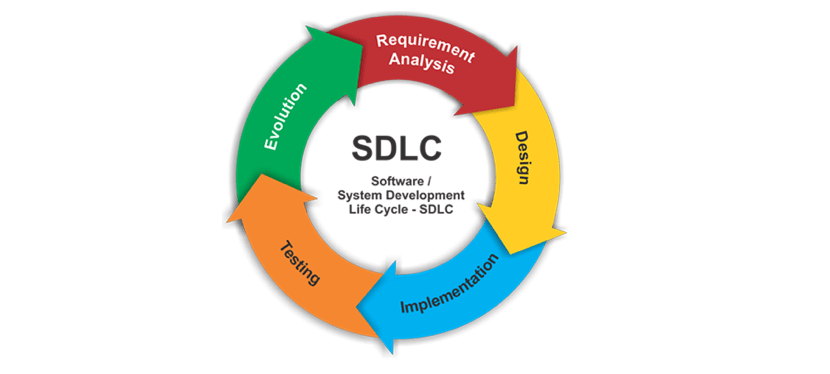
\includegraphics[scale=0.5]{img/SDLC.png}
    \label{fig:SDLC}
    \vspace{0.2cm}
\end{graphic}

\whitespace
In het volgende secties wordt de organisatie beschreven verder wordt de aanleiding en de context van de afstudeeropdracht beschreven.

\section{Organisatieomschrijving}
Je Organisatieomschrijving

\section{Context}
Snakeware heeft een platform genaamd \qw{Snakeware Cloud} dit platform is een \gls{CMS} waarmee ze digitale content kunnen leveren voor haar (grotere) klanten.
Snakeware Cloud is een applicatie waarmee Snakeware en haar klanten webapplicaties kan inrichten en voorzien van content.

\whitespace[2]
De klant van Snakeware kan zijn of haar website zelf inrichten door middel van het specificeren van de content op de verschillende pagina’s.
Dit wordt gedaan door middel van artikelen die door het \gls{CMS} gebruikt kunnen worden.
De content van het artikel kan verschillen tussen simpele tekst, vragenlijst, webshop producten, etc.
Hiernaast zijn er ook \gls{SEO} opties binnen Snakeware Cloud om de site goed te kunnen vinden op het internet.
Hierbij zijn er opties zoals de mogelijkheid om de title tags en zoekwoorden toe te kunnen voegen in de head \Parencite{HTMLhead}

\whitespace[2]
Hierom heeft Snakeware Cloud veel features en configuratie stappen wat het complex en duur maakt om een relatief kleine webapplicatie te maken voor kleinere klanten.
Dit zorgt ervoor dat Snakeware zich niet kan vestigen in een markt met veel kleinere klanten, en hierdoor omzet misloopt.
 % huidige en gewenste situatie
\section{Aanleiding}
Het huidige platform is 21 jaar oud en er is veel functionaliteit in de loop der jaren aan toegevoegd.
Omdat Snakeware Cloud een oud platform is zijn er veel technieken en best practices gebruikt die nu niet meer als optimaal worden beschouwd.
Deze technieken waren erg geïntegreerd in Snakeware Cloud en er is het verleden gekozen om niet de code te herschrijven om het aan de huidige standaarden te voldoen van andere projecten.
Een voorbeeld hiervan is tabel naam prefix afkortingen bij elke kolom zetten, of gigantische C\# \Parencite{CSharp} files van 10 000 regels met verschillende functies.
Deze functies houden zich niet aan de \textit{Single Responsibility Principle} van de SOLID ontwerpmethode \Parencite{SOLID} wat het moeilijk maakt om het huidige \gls{CMS} te onderhouden.

\whitespace
Ook zijn er technieken toegepast die nu niet meer relevant zijn.
Een voorbeeld hiervan is dat het \gls{CMS} gebruikmaakt van JavaScript \Parencite{JavaScript} en toen ze er mee begonnen bestonden JavaScript classes \Parencite{JavascriptClasses} nog niet, dus hebben ze die zelf geïmplementeerd.
Deze oudere technieken en standaarden zorgen ervoor dat het meer tijd kost om het CMS te onderhouden vanwege de extra code.
Dit zorgt ervoor dat het meer tijd en geld kost om het Snakeware Cloud uit te breiden.
% \todo[inline]{ik wou graag bloat gebruiken inplaats van extra code maar volgens kan dat niet suggesities}
% Deze oudere technieken zorgen voor veel overhead en zorgt ervoor dat het veel tijd en geld kost om het \gls{CMS} uit te breiden.

\whitespace[2]
Een van de voornaamste uitdaging met Snakeware Cloud betreft de verouderde datastructuur van de applicatie.
Deze veroudering is het gevolg van een initïele ontwikkeling waarbij onvoldoende rekening werd gehouden met toekomstige functionaliteitsuitbreidingen in het systeem.
Als gevolg daarvan is de onderliggende datastructuur niet aangepast, maar zijn er elementen aan toegevoegd.
Dit heeft geresulteerd in database query's van duizenden regels en complexe relaties tussen tabellen in de database.
Dit huidige scenario bemoeilijkt aanzienlijk het toevoegen van nieuwe functionaliteiten, wat resulteert in aanzienlijke tijd en kosten investeringen.

\newpage
\whitespace
Hierom wil Snakeware een nieuw systeem met een nieuwe datastructuur.
% Hierom wil Snakeware dat er een nieuwe datastructuur komt met de daar bij behoorende \gls{CMS}-API.
Door het gebruiken van een nieuwe softwarearchitectuur zouden er velen problemen opgelost kunnen worden die nu voor komen.
Omdat er een nieuwe datastructuur moet komen en de logica van het oude systeem nauw verbonden is met de datastructuur is het niet mogelijk om de oude code opnieuw te gebruiken.
% \todo[inline]{Dit laatste blokje heb ik aangepast check het later nog een keer na}

\section{Opdrachtomschrijving}
\label{sec:Opdrachtomschrijving}
De opdracht is om een proof of concept CMS-API te ontwikkelen die gebruikt maakt van een datamodel en systeemarchitectuur dat flexibeler, onderhoudbaarder is en gebruik maakt van moderne best practices.
Tijdens de afstudeeropdracht wordt er primair op het datamodel en de systeemarchitectuur gefocust.
Omdat er nog geen concreet datamodel en systeemarchitectuur is zal dit onderzocht en ontworpen moeten worden.

\whitespace[2]
De opdracht omvat het achterhalen van de requirements, ontwerpen en ontwikkelen van het proof of concept met als focus een nieuw datamodel, met de essentiële functionaliteiten.

\whitespace[2]
Het huidige Snakeware Cloud platform bestaat uit 2 verschillende \gls{GUI}:
\begin{itemize}
	\item[-] Snakeware Cloud \gls{GUI}
	\item[-] Klant webapplicatie
\end{itemize}

\whitespace
Met de Snakeware Cloud \gls{GUI} kan de klant de content van de website aanpassen.
Door middel van de webapplicatie kan de eindgebruiker de content bekijken en er mee interacteren.
Er is voor gekozen om niet de Snakeware Cloud \gls{GUI} te realiseren om de afstudeeropdracht in scope te houden.
Er is wel voor gekozen om de klant webapplicatie in zijn minimale vorm uit te werken.
Om de userflows van de applicatie toch te kunnen testen wordt er gebruik gemaakt van postman workflows \Parencite{PostmanWorkflows}

\whitespace[2]
% Om de \gls{UserJourneys} te testen wordt er gebruikgemaakt van postman workflows \Parencite{PostmanWorkflows}.
Het doel van het proof of concept is dat er aangetoond kan worden dat door het gebruiken van een nieuw datamodel en systeemarchitectuur ook services verleend kunnen worden aan kleinere klanten.
Dit zou eventueel ook een startpunt zijn om op verder te bouwen.
% \todo[inline]{Feedback van justin: \textit{Deze paragraaf is nu niet gepast voor een onderzoeksverslag}}
% \todo[inline]{Misschien een stukje theoretisch kader/ voor onderzoek te hebben waarin je het CMS ietwat toelicht (misscien met plaatje wow) (De pre, zonder je deelvragen te beantwoorden). Ik weet alleen niet of ik hier genoeg tijd voor heb}
%

% \section{Stakeholders}
In het vooronderzoek wordt er een stakeholdersanalyse gemaakt om de stakeholders in beeld te krijgen.
De stakeholders zijn individuen of organisaties die invloed of belang hebben bij het project.
De product owner zal de mogelijke markt van kleine klanten representeren.
Dit wordt gedaan omdat Snakeware niet kleine klanten heeft die gebruikt kunnen worden als stakeholders.
% Sommige externe stakeholders zullen gerepresenteerd worden door een gekwalificeerde interne medewerker van Snakeware.
% Dit wordt gedaan omdat de afstudeeropdracht een proof of concept is, en de klanten van Snakeware hier nog niet bij betrokken worden.
Als na de afstudeerperiode het een succes blijkt te zijn en Snakeware wilt het verder ontwikkelen dan wordt contact opgezocht met de externe stakeholders (potentieele kleinere klanten). 
Verder is er een invloed matrix gemaakt (figuur \ref{fig:StakeholdersInvloedMatrix}) om de invloed en belang van de stakeholders te visualiseren. \\
Het project bestaat uit de volgende stakeholders:
\whitespace
\textbf{Product Owner:}
De Product Owner is verantwoordelijk voor het vertegenwoordigen van de belangen, eisen en wensen van de kleinere klanten.
Deze kleinere klanten worden niet als individuele stakeholders beschouwd, aangezien Snakeware geen afzonderlijke kleine klanten heeft.
Om deze reden wordt er binnen Snakeware een gekwalificeerde persoon ingezet om hen te vertegenwoordigen.
\whitespace
\textbf{Afdeling R\&D:} De afdeling R\&D van Snakeware zijn de ontwikkelaars van het huidige \gls{CMS} en kunnen veel inzicht bieden in de huidige situatie / problemen.
\whitespace
Het product bestaat uit twee software-applicaties een frontend die de data weergeeft aan de gebruiker, en een \gls{CMS}-API die de data serveerd voor de frontend.
Deze twee software-applicaties worden na de afstudeerperiode overgedragen aan twee verschillende diseplines in Snakeware, namelijk de backend en frontend developers.
\\
\textbf{Backend developers:} De \gls{CMS}-API wordt aan het einde van de afstudeeropdracht overgedragen aan de backend developers van Snakeware.
Tijdens de ontwerp en realisatie fase kan er voor advies gevraagd worden over hoe de \gls{CMS}-API het best ontworpen / gerealiseerd kan worden. \\
\textbf{Frontend developers} : De interface applicatie die gemaakt wordt om de data te tonen aan de gebruiker wordt ook overgedragen aan het einde van de afstudeeropdracht.
Tijdens de ontwerp en realisatie fase kan er voor advies gevraagd worden over hoe de inteface het best ontworpen / gerealiseerd kan worden.
\begin{graphic}
    \captionsetup{type=figure}
    \caption{Stakeholders invloed matrix}
    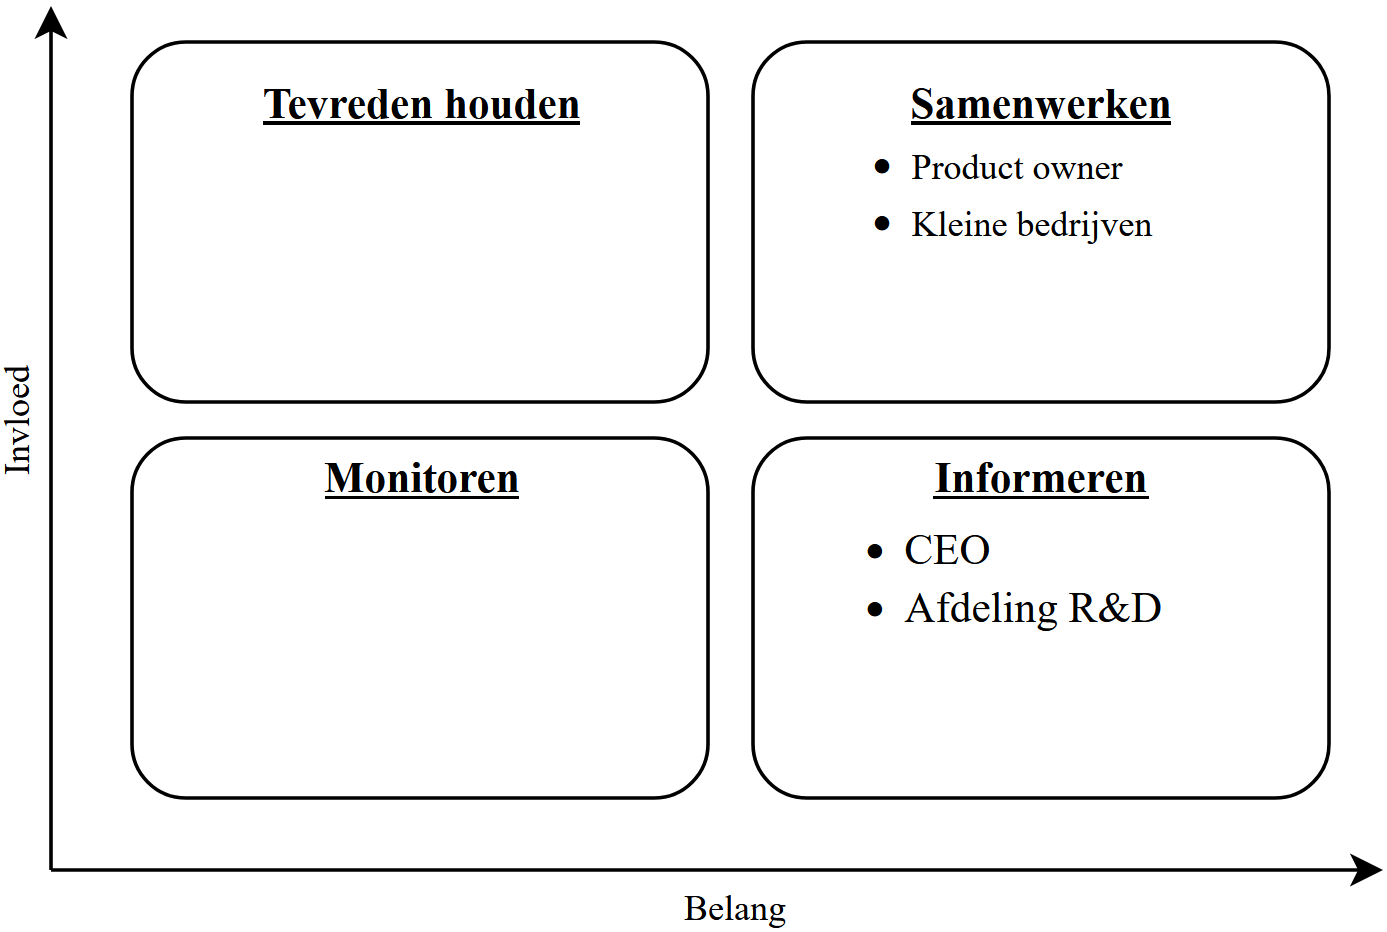
\includegraphics[scale=0.4]{StakeholdersInvloedMatrix}
    \label{fig:StakeholdersInvloedMatrix}
\end{graphic}

\section{Leeswijzer}
In hoofdstuk 2 wordt de onderzoeksopzet behandeld hier worden de hoofd- en deelvraag opgesteld.
Daarnaast worden de verschillende onderzoeksmethoden uitgelegd bij elke deelvraag.
In hoofdstuk 3 worden de resultaten van het onderzoek behandeld en geanalyseerd.
In hoofdstuk 4 wordt de conclusie van het onderzoek behandeld en wordt er antwoord gegeven op de hoofdvraag.
In het laatste hoofdstuk wordt de discussie en reflectie behandeld.

